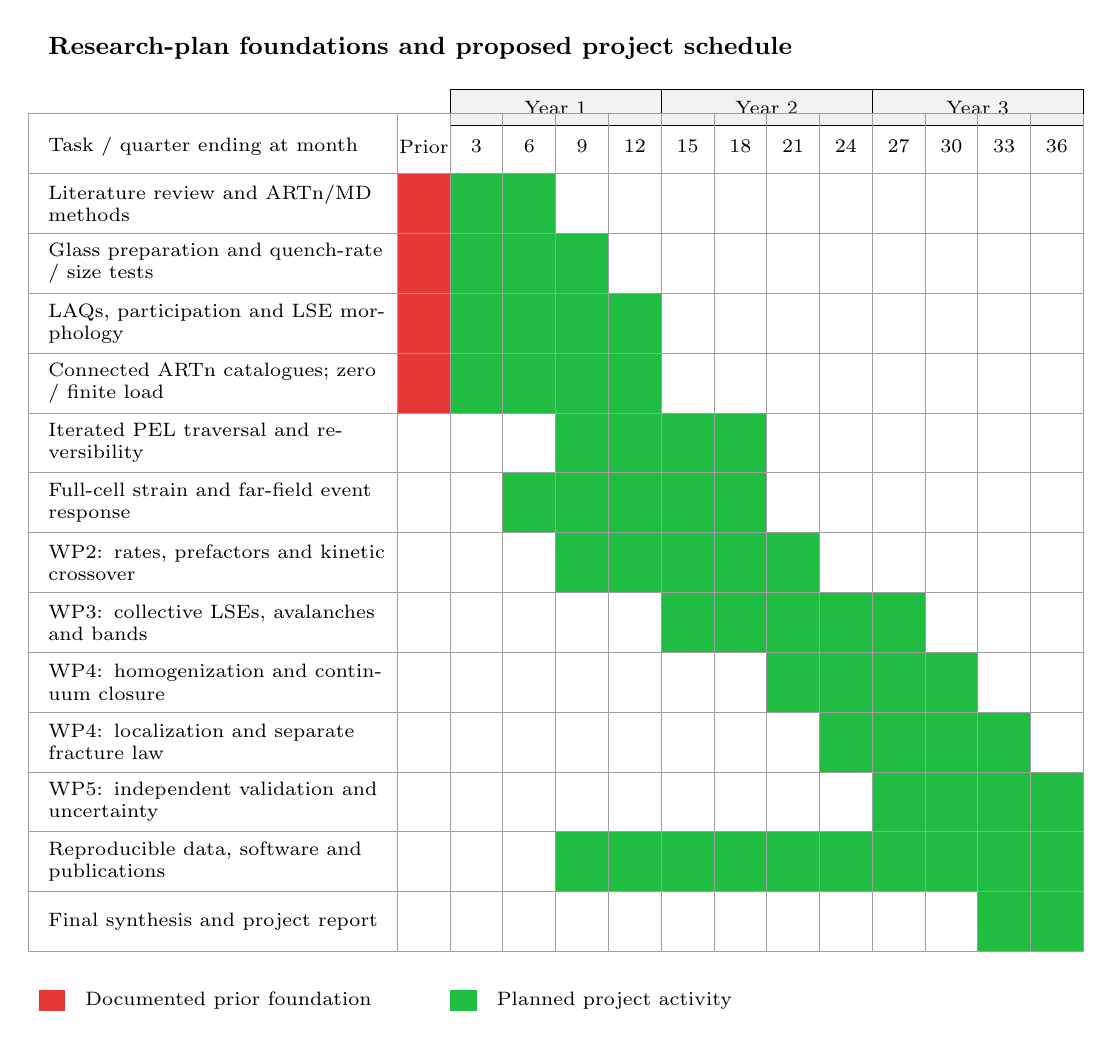
\begin{tikzpicture}[x=0.67cm,y=0.76cm,font=\scriptsize]
\definecolor{planred}{HTML}{E53935}
\definecolor{plangreen}{HTML}{21BC42}
\node[anchor=west,font=\small\bfseries] at (-6.8,2.1) {Research-plan foundations and proposed project schedule};
\draw[fill=gray!10] (1,0.8) rectangle (5,1.4);
\node at (3.0,1.1) {Year 1};
\draw[fill=gray!10] (5,0.8) rectangle (9,1.4);
\node at (7.0,1.1) {Year 2};
\draw[fill=gray!10] (9,0.8) rectangle (13,1.4);
\node at (11.0,1.1) {Year 3};
\node at (0.5,0.45) {Prior};
\node[anchor=west] at (-6.8,0.45) {Task / quarter ending at month};
\node at (1.5,0.45) {3};
\node at (2.5,0.45) {6};
\node at (3.5,0.45) {9};
\node at (4.5,0.45) {12};
\node at (5.5,0.45) {15};
\node at (6.5,0.45) {18};
\node at (7.5,0.45) {21};
\node at (8.5,0.45) {24};
\node at (9.5,0.45) {27};
\node at (10.5,0.45) {30};
\node at (11.5,0.45) {33};
\node at (12.5,0.45) {36};
\fill[planred] (0,0) rectangle (1,-1);
\fill[plangreen] (1,0) rectangle (2,-1);
\fill[plangreen] (2,0) rectangle (3,-1);
\node[anchor=west,text width=4.35cm,align=left] at (-6.8,-0.5) {Literature review and ARTn/MD methods};
\fill[planred] (0,-1) rectangle (1,-2);
\fill[plangreen] (1,-1) rectangle (2,-2);
\fill[plangreen] (2,-1) rectangle (3,-2);
\fill[plangreen] (3,-1) rectangle (4,-2);
\node[anchor=west,text width=4.35cm,align=left] at (-6.8,-1.5) {Glass preparation and quench-rate / size tests};
\fill[planred] (0,-2) rectangle (1,-3);
\fill[plangreen] (1,-2) rectangle (2,-3);
\fill[plangreen] (2,-2) rectangle (3,-3);
\fill[plangreen] (3,-2) rectangle (4,-3);
\fill[plangreen] (4,-2) rectangle (5,-3);
\node[anchor=west,text width=4.35cm,align=left] at (-6.8,-2.5) {LAQs, participation and LSE morphology};
\fill[planred] (0,-3) rectangle (1,-4);
\fill[plangreen] (1,-3) rectangle (2,-4);
\fill[plangreen] (2,-3) rectangle (3,-4);
\fill[plangreen] (3,-3) rectangle (4,-4);
\fill[plangreen] (4,-3) rectangle (5,-4);
\node[anchor=west,text width=4.35cm,align=left] at (-6.8,-3.5) {Connected ARTn catalogues; zero / finite load};
\fill[plangreen] (3,-4) rectangle (4,-5);
\fill[plangreen] (4,-4) rectangle (5,-5);
\fill[plangreen] (5,-4) rectangle (6,-5);
\fill[plangreen] (6,-4) rectangle (7,-5);
\node[anchor=west,text width=4.35cm,align=left] at (-6.8,-4.5) {Iterated PEL traversal and reversibility};
\fill[plangreen] (2,-5) rectangle (3,-6);
\fill[plangreen] (3,-5) rectangle (4,-6);
\fill[plangreen] (4,-5) rectangle (5,-6);
\fill[plangreen] (5,-5) rectangle (6,-6);
\fill[plangreen] (6,-5) rectangle (7,-6);
\node[anchor=west,text width=4.35cm,align=left] at (-6.8,-5.5) {Full-cell strain and far-field event response};
\fill[plangreen] (3,-6) rectangle (4,-7);
\fill[plangreen] (4,-6) rectangle (5,-7);
\fill[plangreen] (5,-6) rectangle (6,-7);
\fill[plangreen] (6,-6) rectangle (7,-7);
\fill[plangreen] (7,-6) rectangle (8,-7);
\node[anchor=west,text width=4.35cm,align=left] at (-6.8,-6.5) {WP2: rates, prefactors and kinetic crossover};
\fill[plangreen] (5,-7) rectangle (6,-8);
\fill[plangreen] (6,-7) rectangle (7,-8);
\fill[plangreen] (7,-7) rectangle (8,-8);
\fill[plangreen] (8,-7) rectangle (9,-8);
\fill[plangreen] (9,-7) rectangle (10,-8);
\node[anchor=west,text width=4.35cm,align=left] at (-6.8,-7.5) {WP3: collective LSEs, avalanches and bands};
\fill[plangreen] (7,-8) rectangle (8,-9);
\fill[plangreen] (8,-8) rectangle (9,-9);
\fill[plangreen] (9,-8) rectangle (10,-9);
\fill[plangreen] (10,-8) rectangle (11,-9);
\node[anchor=west,text width=4.35cm,align=left] at (-6.8,-8.5) {WP4: homogenization and continuum closure};
\fill[plangreen] (8,-9) rectangle (9,-10);
\fill[plangreen] (9,-9) rectangle (10,-10);
\fill[plangreen] (10,-9) rectangle (11,-10);
\fill[plangreen] (11,-9) rectangle (12,-10);
\node[anchor=west,text width=4.35cm,align=left] at (-6.8,-9.5) {WP4: localization and separate fracture law};
\fill[plangreen] (9,-10) rectangle (10,-11);
\fill[plangreen] (10,-10) rectangle (11,-11);
\fill[plangreen] (11,-10) rectangle (12,-11);
\fill[plangreen] (12,-10) rectangle (13,-11);
\node[anchor=west,text width=4.35cm,align=left] at (-6.8,-10.5) {WP5: independent validation and uncertainty};
\fill[plangreen] (3,-11) rectangle (4,-12);
\fill[plangreen] (4,-11) rectangle (5,-12);
\fill[plangreen] (5,-11) rectangle (6,-12);
\fill[plangreen] (6,-11) rectangle (7,-12);
\fill[plangreen] (7,-11) rectangle (8,-12);
\fill[plangreen] (8,-11) rectangle (9,-12);
\fill[plangreen] (9,-11) rectangle (10,-12);
\fill[plangreen] (10,-11) rectangle (11,-12);
\fill[plangreen] (11,-11) rectangle (12,-12);
\fill[plangreen] (12,-11) rectangle (13,-12);
\node[anchor=west,text width=4.35cm,align=left] at (-6.8,-11.5) {Reproducible data, software and publications};
\fill[plangreen] (11,-12) rectangle (12,-13);
\fill[plangreen] (12,-12) rectangle (13,-13);
\node[anchor=west,text width=4.35cm,align=left] at (-6.8,-12.5) {Final synthesis and project report};
\draw[gray!75,line width=0.3pt] (-7,1) -- (13,1);
\draw[gray!75,line width=0.3pt] (-7,0) -- (13,0);
\draw[gray!75,line width=0.3pt] (-7,-1) -- (13,-1);
\draw[gray!75,line width=0.3pt] (-7,-2) -- (13,-2);
\draw[gray!75,line width=0.3pt] (-7,-3) -- (13,-3);
\draw[gray!75,line width=0.3pt] (-7,-4) -- (13,-4);
\draw[gray!75,line width=0.3pt] (-7,-5) -- (13,-5);
\draw[gray!75,line width=0.3pt] (-7,-6) -- (13,-6);
\draw[gray!75,line width=0.3pt] (-7,-7) -- (13,-7);
\draw[gray!75,line width=0.3pt] (-7,-8) -- (13,-8);
\draw[gray!75,line width=0.3pt] (-7,-9) -- (13,-9);
\draw[gray!75,line width=0.3pt] (-7,-10) -- (13,-10);
\draw[gray!75,line width=0.3pt] (-7,-11) -- (13,-11);
\draw[gray!75,line width=0.3pt] (-7,-12) -- (13,-12);
\draw[gray!75,line width=0.3pt] (-7,-13) -- (13,-13);
\draw[gray!75,line width=0.3pt] (-7,1) -- (-7,-13);
\draw[gray!75,line width=0.3pt] (0,1) -- (0,-13);
\draw[gray!75,line width=0.3pt] (1,1) -- (1,-13);
\draw[gray!75,line width=0.3pt] (2,1) -- (2,-13);
\draw[gray!75,line width=0.3pt] (3,1) -- (3,-13);
\draw[gray!75,line width=0.3pt] (4,1) -- (4,-13);
\draw[gray!75,line width=0.3pt] (5,1) -- (5,-13);
\draw[gray!75,line width=0.3pt] (6,1) -- (6,-13);
\draw[gray!75,line width=0.3pt] (7,1) -- (7,-13);
\draw[gray!75,line width=0.3pt] (8,1) -- (8,-13);
\draw[gray!75,line width=0.3pt] (9,1) -- (9,-13);
\draw[gray!75,line width=0.3pt] (10,1) -- (10,-13);
\draw[gray!75,line width=0.3pt] (11,1) -- (11,-13);
\draw[gray!75,line width=0.3pt] (12,1) -- (12,-13);
\draw[gray!75,line width=0.3pt] (13,1) -- (13,-13);
\fill[planred] (-6.8,-14) rectangle (-6.3,-13.65);
\node[anchor=west] at (-6.1,-13.82) {Documented prior foundation};
\fill[plangreen] (1,-14) rectangle (1.5,-13.65);
\node[anchor=west] at (1.7,-13.82) {Planned project activity};
\end{tikzpicture}